\documentclass[11pt]{beamer}
\usepackage{hyperref}
\usepackage[T1]{fontenc}
\UseRawInputEncoding

\usepackage{graphicx}
\usepackage[utf8]{inputenc}
\usepackage{mathtools}
\usepackage{verbatim}
\usepackage{smartdiagram}
\usepackage{unicode-math}
%\setmathfont{}
\usepackage{comment}
\usepackage{xcolor}
% Cannot enable in Xelatex
\usepackage{pgfpages}
% \setbeameroption{hide notes} % Only slides
% \setbeameroption{show only notes} % Only notes
% \setbeameroption{show notes on second screen}
\usepackage{latexsym,amsmath,xcolor,multicol,booktabs,calligra}
\usepackage{graphicx,listings,stackengine}

\usepackage{tikz}
\usepackage{tikz-feynman}
\usepackage[compat=1.0.0]{tikz-feynman}
\usepackage{float}

%% Enable only in Xelatex
% \usepackage{pstricks}
\usepackage{feynmp-auto} % or feynmp if you prefer
% Feynman diagrams
%\usepackage{feynmp}
%\usepackage{feynmf}
\DeclareGraphicsRule{*}{mps}{*}{} % for being able to read the produced file

\author{Ana Costa Pereira, Martin Gorbahn, Francesco Moretti, Kai Sieja, Emmanuele Stamou}
\title{Universal Radiative Corrections for Precision
Determinations of $V_{ud}$}
\institute [University of Liverpool] {\href{mailto:Ana.Costa-Pereira@liverpool.ac.uk}{\underline{Ana.Costa-Pereira@liverpool.ac.uk}}}
\date{08/06/2026}
\usepackage{QUT}

% defs
\def\cmd#1{\texttt{\color{red}\footnotesize $\backslash$#1}}
\def\env#1{\texttt{\color{blue}\footnotesize #1}}
\definecolor{deepblue}{rgb}{0,0,0.5}
\definecolor{deepred}{rgb}{0.6,0,0}
\definecolor{deepgreen}{rgb}{0,0.5,0}
\definecolor{halfgray}{gray}{0.55}

\lstset{
    basicstyle=\ttfamily\small,
    keywordstyle=\bfseries\color{deepblue},
    emphstyle=\ttfamily\color{deepred},    % Custom highlighting style
    stringstyle=\color{deepgreen},
    numbers=left,
    numberstyle=\small\color{halfgray},
    rulesepcolor=\color{red!20!green!20!blue!20},
    frame=shadowbox,
}

\setbeamercolor{block body alerted}{bg=alerted text.fg!10}
\setbeamercolor{block title alerted}{bg=alerted text.fg!20}
\setbeamercolor{block body}{bg=structure!10}
\setbeamercolor{block title}{bg=structure!20}
\setbeamercolor{block body example}{bg=green!10}
\setbeamercolor{block title example}{bg=green!20}

\begin{document}
%
%
% Capa
%
%
\begin{frame}
    \titlepage

    \begin{columns}[c]
        \column{0.5\textwidth}
        \centering
        
\includegraphics[width=0.7\linewidth]{logo.png}

        \column{0.5\textwidth}
        \centering
        
\includegraphics[width=0.7\linewidth]{logo_livinno.jpg}
    \end{columns}
\end{frame}


\begin{frame}
    \tableofcontents[sectionstyle=show,subsectionstyle=show/shaded/hide,subsubsectionstyle=show/shaded/hide]
\end{frame}













\begin{frame}
\begin{itemize}
\item SM shortcomings: Origin of flavour, CP problem, dark energy, dark matter, matter/anti-matter asymmetry;
\item CKM (mixing of quark flavour eigenstates) tested at level $0.01\%$;
\item Cabbibo angle anomaly;
\item Measure decay rates: $K$, $0^+ \longrightarrow 0^+$, $\Pi$, neutron decay;
\item Semileptonic decays: $K_{l3}$, $0^+ \longleftarrow 0^+$, neutron decay;
\item Leptonic decays:  $K_{l2}$;
\item Status of $V_{ud}$, $V_{us}$;
\end{itemize}

\end{frame}






\section{Semi-leptonic kaon decays}

\begin{frame}{$K_{l3}$ - Semi-leptonic kaon decays}
\begin{equation*}
\Gamma\!\left(K_{\ell3}\right)
=
\frac{G_F^2 M_K^5}{192\pi^3}\,
C_K^2\,
S_{\mathrm{EW}}\,
|V_{us}|^2\,
\bigl|f_+^{K^0\pi^-}(0)\bigr|^2\,
I_{K\ell}^{(0)}
\left(
1+\delta_{SU(2)}^{K\pi}
+\delta_{\mathrm{EM}}^{K\ell}
\right)^2 
\end{equation*}
\begin{itemize}
\item $S_{EW} = 1.0232(3) \longrightarrow$ process indepented EW corrections;
\item $I_{K\ell}^{(0)}$ phase space in isospin limit;
\item $\delta_{SU(2)}^{K\pi}$ strong isospin breakig correction
\item $\delta_{\mathrm{EM}}^{K\ell}$ long distance EW corrections
\end{itemize}
\textbf{Experimental inputs}
\[
|V_{us}|\,f_+(0)=0.21654(41)
\]

\end{frame}











\begin{frame}
\begin{figure}
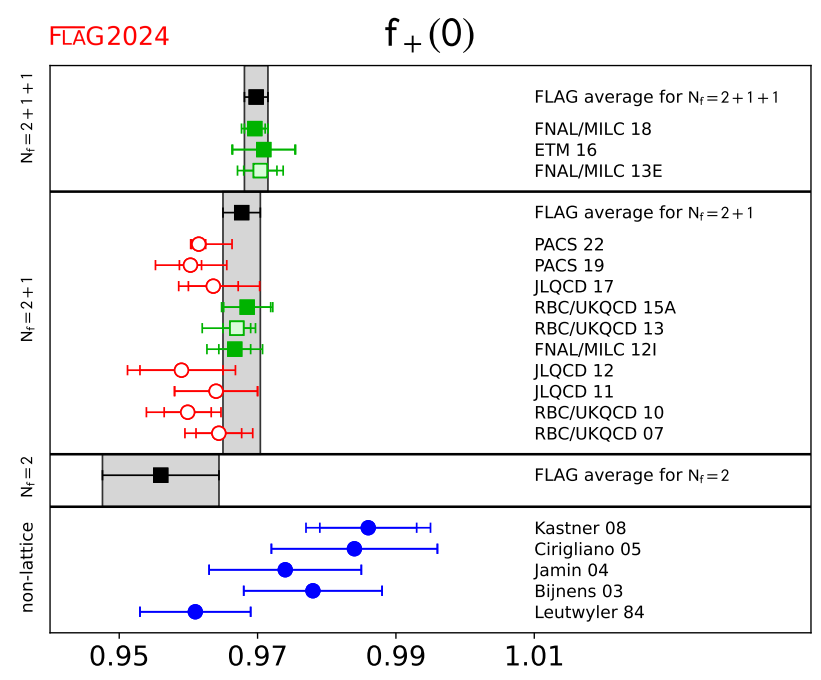
\includegraphics[scale=.25]{flag1.png}
\end{figure}
\[
f_+(0)=0.9698(17)
\]

\[
|V_{us}| = 0.22328(58)
\qquad (K_{\ell3})
\]
\end{frame}





\section{Ratio of $V_{us}/V_{ud}$}

\begin{frame}
\begin{equation*}
\frac{\Gamma(K^\pm_{\mu2(\gamma)})}
     {\Gamma(\pi^\pm_{\mu2(\gamma)})}
=
\left|\frac{V_{us}}{V_{ud}}\right|^2
\left(\frac{f_{K^\pm}}{f_{\pi^\pm}}\right)^2
\frac{M_{K^\pm}\left(1-m_\mu^2/M_{K^\pm}^2\right)^2}
     {M_{\pi^\pm}\left(1-m_\mu^2/M_{\pi^\pm}^2\right)^2}
\left(1+\delta_{\rm EM}\right)
\end{equation*}

\textbf{Experimental inputs}
\[
\left|\frac{V_{us}}{V_{ud}}\right|
\frac{f_{K^\pm}}{f_{\pi^\pm}}
=
0.27599(41)
\]

\[
|V_{ud}|=0.97373(31)
\qquad
(\text{superallowed }\beta\text{ decays})
\]
\end{frame}










\begin{frame}
\begin{figure}
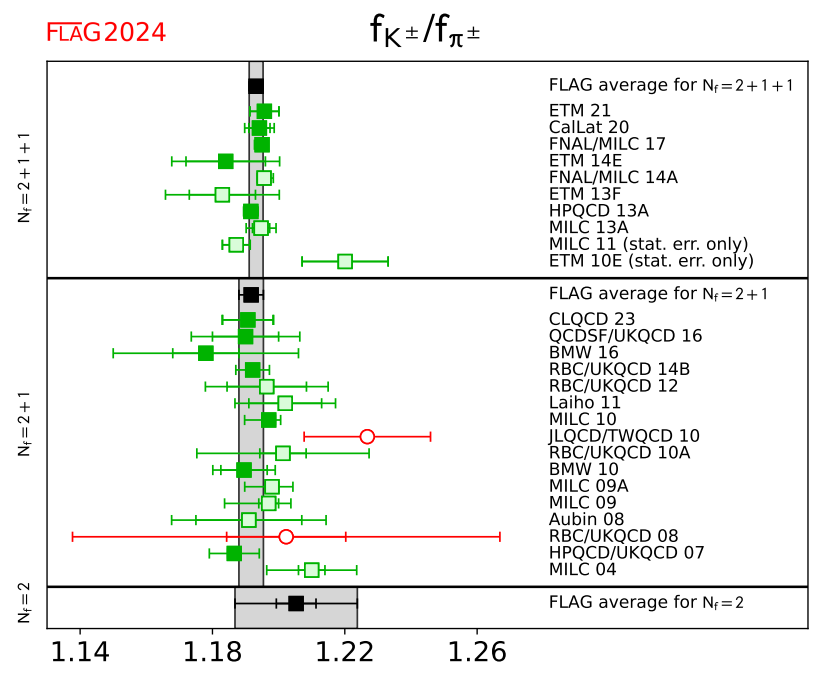
\includegraphics[scale=.25]{flag.png}
\end{figure}
\small
\[
\frac{f_{K^\pm}}{f_{\pi^\pm}}
=
1.1934(19)
\]



\[
\left|\frac{V_{us}}{V_{ud}}\right|
=
0.23126(50)
\qquad (K_{\ell2}/\pi_{\ell2})
\]

\end{frame}








\begin{frame}{CKM matrix}
\begin{figure}
    \centering
    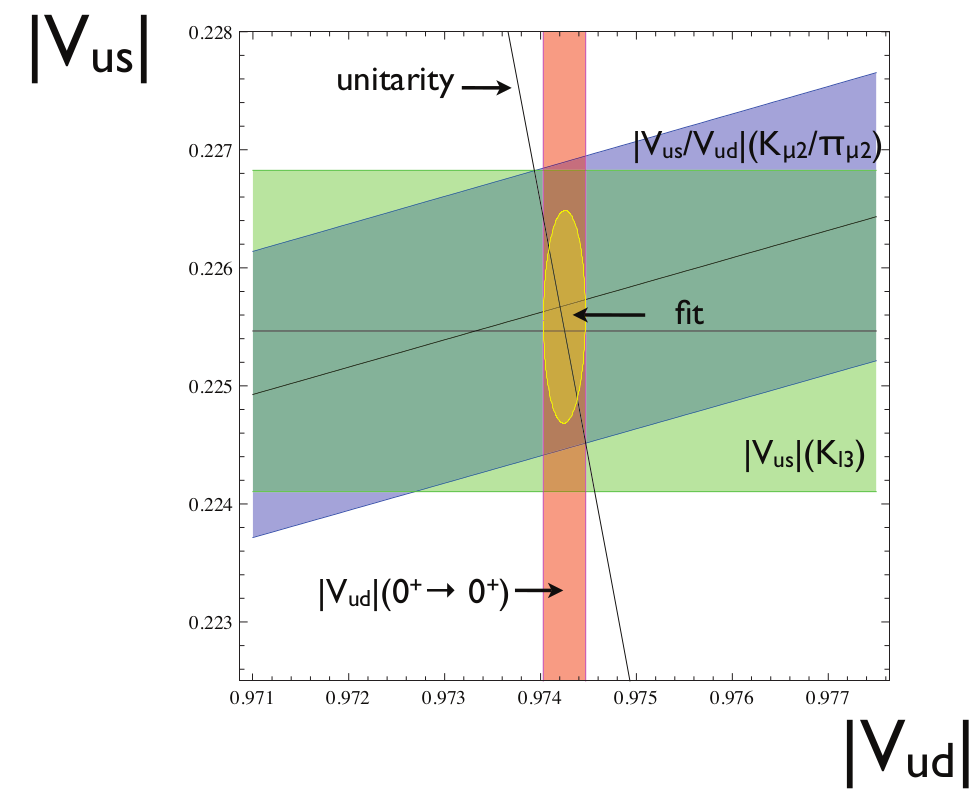
\includegraphics[scale=.2]{flagcomb.png}
\end{figure}
\begin{equation}
   |V_{ud}|^2 + |V_{us}|^2- O|V_{ub}|^2 = 1
\end{equation}
\end{frame}














\section{Radiative corrections and EFT formalism}

\begin{frame}{Operator product expansion}
\begin{figure}[H]
\centering

% ---- First Minipage ----
\begin{minipage}[b]{0.4\linewidth}
\centering
\vspace{.2cm}
\resizebox{0.6\linewidth}{!}{ % scale to 90% of minipage width
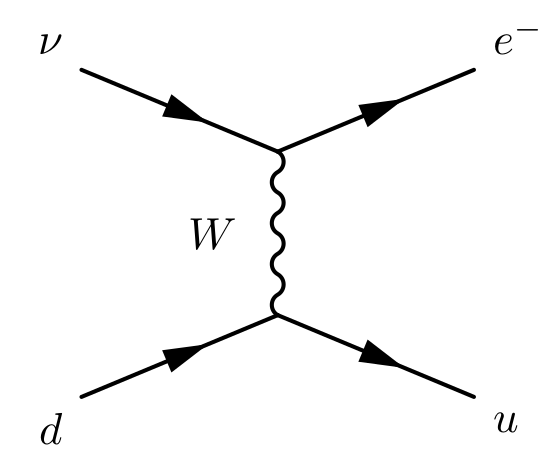
\includegraphics[scale=.5]{full.png}
}
\vspace{.2cm}
\caption{SM tree-level.}
\label{treelevelfull}
\end{minipage}
\hfill
\begin{minipage}[b]{0.4\linewidth}
\centering
\vspace{.2cm}
\resizebox{0.6\linewidth}{!}{ % scale to 90% of minipage width
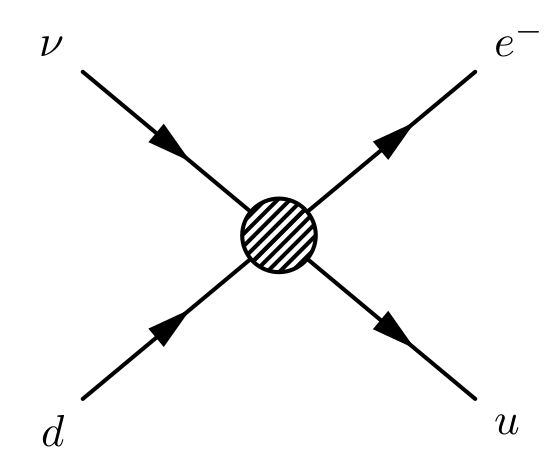
\includegraphics[scale=.5]{eft.png}
}
\caption{EFT Tree-level.}
\label{treeleveleft}
\end{minipage}
\end{figure}

\begin{equation}
     \frac{1}{k^2-m_W^2} \longrightarrow \frac{-1}{m_W^2}
\end{equation}

\begin{equation}
    H_{eff}(x) = \dfrac{G_F}{\sqrt{2}} V_{CKM}^{i} C_i(\mu) Q_i(x)
\end{equation}


\end{frame}


















\section{NLO EW corrections}

\begin{frame}{NLO EW corrections}
\begin{figure}[h]
\centering
\begin{minipage}[c]{0.45\textwidth}
\begin{tikzpicture}
\begin{feynman}
\vertex (u) at (0,1.5) {\(u\)};
\vertex (a) at (1.5,1.5);
\vertex (d) at (3,1.5) {\(d\)};
\vertex (c1) at (1.5,0.975);
\vertex (c2) at (1.5,0.525);
\vertex (c) at (1.5,0);
\vertex (e) at (0,0) {\(e\)};
\vertex (ve) at (3,0) {\(\nu_e\)};
\diagram* {
  (u) -- [fermion] (a) -- [fermion] (d),
  (a) -- [boson, edge label=\(W\)] (c1),
  (c1) -- [fermion, half left, looseness=1.4, edge label=\(b\)] (c2)
        -- [fermion, half left, looseness=1.4, edge label=\(t\)] (c1),
  (c2) -- [boson, edge label=\(W\)] (c),
  (e) -- [fermion] (c) -- [fermion] (ve),
};
\end{feynman}
\end{tikzpicture}
\end{minipage}
\hfill
\begin{minipage}[c]{0.45\textwidth}
\begin{tikzpicture}
\begin{feynman}
\vertex (u) at (0,1.5) {\(u\)};
\vertex (a) at (1,1.5);
\vertex (a1) at (2,1.5);
\vertex (d) at (3,1.5) {\(d\)};
\vertex (e) at (0,0) {\(e\)};
\vertex (c) at (1,0);
\vertex (c1) at (2,0);
\vertex (ve) at (3,0) {\(\nu_e\)};
\diagram* {
  (u) -- [fermion] (a) -- [fermion, edge label=\(u\)] (a1) -- [fermion] (d),
  (a) -- [boson, edge label'=\(Z\)] (c),
  (a1) -- [boson, edge label=\(W\)] (c1),
  (e) -- [fermion] (c)  -- [fermion, edge label'=\(e\)] (c1) -- [fermion] (ve),
};
\end{feynman}
\end{tikzpicture}
\end{minipage}
%\caption{Some 1 loop diagrams in the full theory for the semi-leptonic decay.}
\label{1loopdiag}
\end{figure}


\begin{figure}[h]
\centering
\begin{minipage}[c]{0.45\textwidth}
\begin{tikzpicture}
\begin{feynman}
\vertex (u) at (0,1.5) {\(u\)};
\vertex (a) at (1,1.5);
\vertex (a1) at (2,1.5);
\vertex (d) at (3,1.5) {\(d\)};
\vertex (e) at (0,0) {\(e\)};
\vertex (c) at (1.5,0);
\vertex (c1) at (1.5,0.6);
\vertex (ve) at (3,0) {\(\nu_e\)};
\diagram* {
  (u) -- [fermion] (a) -- [fermion, edge label=\(d\)] (a1) -- [fermion] (d),
  (a) -- [boson, edge label'=\(W\)] (c1),
  (a1) -- [boson, edge label=\(\gamma\)] (c1),
  (c1) -- [boson, edge label=\(W\)] (c),
  (e) -- [fermion] (c) -- [fermion] (ve),
};
\end{feynman}
\end{tikzpicture}
\end{minipage}
\hfill
\begin{minipage}[c]{0.45\textwidth}
\begin{tikzpicture}
\begin{feynman}
\vertex (u) at (0,1.5) {\(u\)};
\vertex (a) at (1.5,1.5);
\vertex (d) at (3,1.5) {\(d\)};
\vertex (c1) at (1.5,0.75);
\vertex (c2) at (2,0.75);
\vertex (c3) at (2.4,0.75);
\vertex (c) at (1.5,0);
\vertex (e) at (0,0) {\(e\)};
\vertex (ve) at (3,0) {\(\nu_e\)};
\diagram* {
  (u) -- [fermion] (a) -- [fermion] (d),
  (a) -- [boson, edge label'=\(W\)] (c),
  (c1) -- [scalar, edge label=\(H\)] (c2)
        -- [fermion, half left, looseness=1.4] (c3)
        -- [fermion, half left, looseness=1.4, edge label=\(W\)] (c2),
  (e) -- [fermion] (c) -- [fermion] (ve),
};
\end{feynman}
\end{tikzpicture}
\end{minipage}
\caption{Some 1 loop diagrams in the full theory for the semi-leptonic decay.}
\label{1loopdiag}
\end{figure}
\end{frame}


















\begin{frame}{Normalization to $G_F$}
Normalization to $G_F$
\begin{equation}
  \mathcal{L}_{G_F} = -\frac{G_F}{\sqrt{2}} Q_\mu -\frac{G_F}{\sqrt{2}} V_{ud} C_{q} Q_q
\end{equation}

And the Wilson Coefficients are

\begin{align}
  C_{r}^{{LO}}  = 1
\end{align}

\begin{equation}
  C^{NLO}_r = -5 +\frac{a^1_\mu}{4}+\frac{a^1_q}{12} - 2\log\left( \frac{\mu^2}{M_Z^2} \right)\,.
\end{equation}

\begin{itemize}
    \item Finite, scheme dependent ($a_\mu^1$, $a_q^1$)
    \item Only box diagrams contribute
\end{itemize}
\end{frame}













\section{NNLO EW corrections}


\begin{frame}
\begin{figure}
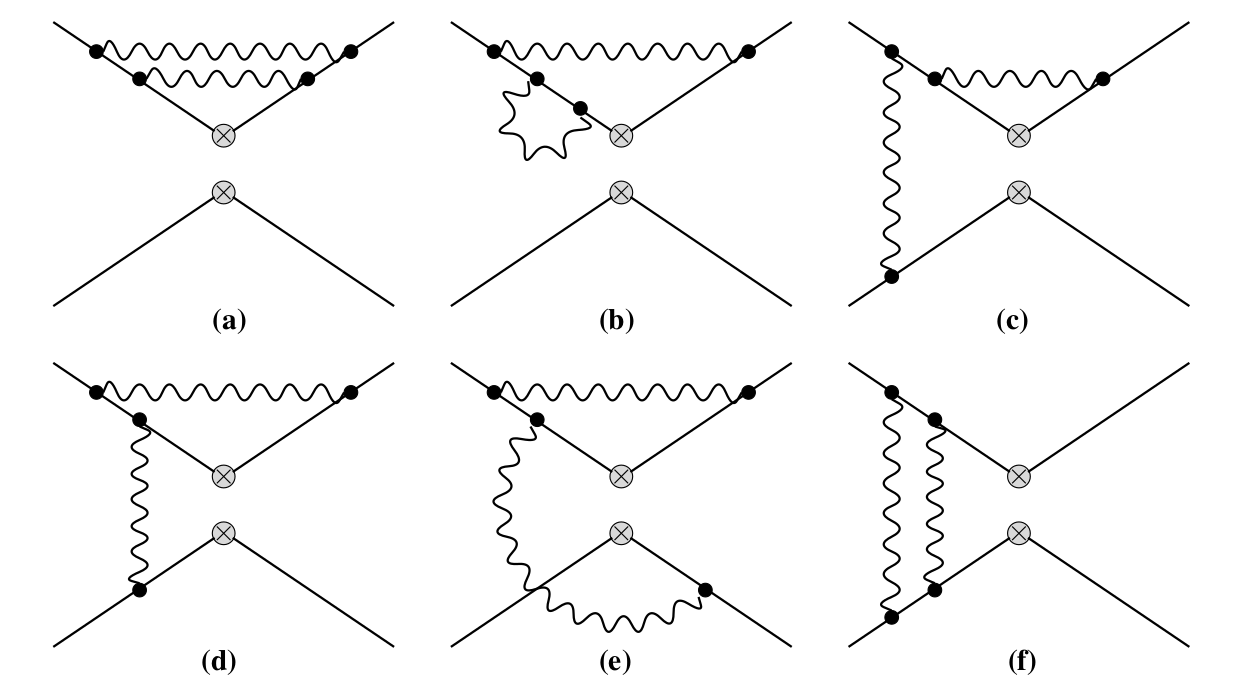
\includegraphics[scale=.15]{eft2l.png}
\caption{EFT NNLO EW corrections.}
\end{figure}
\begin{figure}[h]
\centering

\begin{minipage}{0.48\textwidth}
\centering
\begin{tikzpicture}
\begin{feynman}
\vertex (u) at (0,1.5) {\(u\)};
\vertex (a) at (1,1.5);
\vertex (a1) at (2,1.5);
\vertex (a2) at (3,1.5);
\vertex (d) at (4,1.5) {\(d\)};

\vertex (e) at (0,0) {\(e\)};
\vertex (c) at (1,0);
\vertex (c1) at (2,0);
\vertex (c2) at (3,0);
\vertex (ve) at (4,0) {\(\nu_e\)};

\diagram* {
  (u) -- [fermion] (a) -- [fermion, edge label=\(u\)] (a1) -- [fermion, edge label=\(u\)] (a2) -- [fermion] (d),
  (a) -- [boson, edge label'=\(Z\)] (c),
  (a1) -- [boson, edge label=\(Z\)] (c1),
  (a2) -- [boson, edge label=\(W\)] (c2),
  (e) -- [fermion] (c) -- [fermion, edge label'=\(e\)] (c1)
      -- [fermion, edge label'=\(e\)] (c2) -- [fermion] (ve),
};
\end{feynman}
\end{tikzpicture}

\end{minipage}
\hfill
\begin{minipage}{0.48\textwidth}
\centering
\begin{tikzpicture}
\begin{feynman}
\vertex (u) at (0,1.5) {\(u\)};
\vertex (a) at (1,1.5);
\vertex (a1) at (2,1.5);
\vertex (d) at (3,1.5) {\(d\)};
\vertex (a2) at (1.3,1);
\vertex (a3) at (1.7,1);

\vertex (e) at (0,0) {\(e\)};
\vertex (c) at (1.5,0);
\vertex (c1) at (1.5,0.4);
\vertex (ve) at (3,0) {\(\nu_e\)};

\diagram* {
  (u) -- [fermion] (a) -- [fermion, edge label=\(u\)] (a1) -- [fermion] (d),
  (a) -- [boson, edge label'=\(\gamma\)] (a2) -- [fermion, edge label'=\(e\)] (c1),
  (a1) -- [boson, edge label=\(W\)] (a3) -- [fermion, edge label=\(\nu_e\)] (c1),
  (a2) -- [fermion, edge label=\(e\)] (a3),
  (c1) -- [boson, edge label=\(W\)] (c),
  (e) -- [fermion] (c) -- [fermion] (ve),
};
\end{feynman}
\end{tikzpicture}


\end{minipage}

\caption{SM NNLO EW corrections.}
\end{figure}
\end{frame}


















\begin{frame}{WC and RGE}
RGE for WC:

\begin{equation}
\mu \frac{d}{d\mu} C^f_i(\mu)
=
\sum_j \gamma^f_{ij} \, C^f_j(\mu),
\end{equation}

\begin{equation}
C^{(f)}(\mu)
=
J_f(\mu)\,
U_f(\mu)\,
U_f^{-1}(\mu_0)\,
J_f^{-1}(\mu_0)\,
C^{(f)}(\mu_0)
\end{equation}

insert graph with scale dependence

\end{frame}











\begin{frame}{Conclusions}
    \begin{itemize}
        \item Combination of lattice inputs and perturbative calculations;
        \item Higher order calculation + sub-percent lattice calculations;
        \item Current ongoing work on NNLO EW corrections for $V_{ud}$ extraction from neutron decay. 
    \end{itemize}
\end{frame}










\small
    \bibliographystyle{apalike}
%\printbibliography
\bibliography{slide}
\begin{comment}

\begin{frame}{Physical and Evanescent operator}
        In our case the relevant operators for the pion decay are a physical operator $Q(x)$

\begin{equation}
    Q(x) = (\Bar{d}(x) \gamma^{\mu} P_L u(x) ) (\Bar{\nu}(x) \gamma^{\mu} P_L e(x) ),     \space P_L = \dfrac{1 - \gamma_5}{2}
\end{equation}
\\
and an evanescent operator that can be related with the physical operator

\begin{equation}
E(x) = (\overline{d}(x) \gamma^\mu \gamma^\nu \gamma^\beta P_L u(x)) (\overline{\nu}(x) \gamma_\mu \gamma_\nu \gamma_\beta P_L l(x))
      - (16- a^1_q)  Q(x)
\end{equation}
which vanishes in 4 dimension.
\end{frame}

\begin{frame}{Results for the 1-loop EFT EW corrections for the semi-leptonic decay}
    The sum of the amplitudes $M$ of the 1-loop diagrams of the EFT 
\begin{equation}
    M_{EFT} = \int_k \frac{1}{(k^2-\mu^2)^2}(a_1 Q + a_2 E)
\end{equation}

with 

\begin{equation*}
\begin{split}
   &  a_1 = 
    \frac{\alpha}{4 \pi} G_F \Bigg( Q_u Q_d (\frac{(2-d)^2}{d} - (1 - \xi)) +
     Q_u Q_e (\frac{16}{d} - (1 - \xi))\\
     & + 
     Q_d Q_e (\frac{6d-20}{d} - (1 - \xi)) \Bigg)
\end{split}
\end{equation*}

\begin{equation*}
    a_2 = \frac{\alpha}{4 \pi} \frac{G_F}{d} \Big( Q_u Q_e - Q_d Q_e \Big)
\end{equation*}

with $Q_u$, $Q_d$, $Q_e$ being respectively the quark up, down and electron charges, $\alpha = \frac{e^2}{4 \pi}$ and $\xi$ is the Gauge of the photon.
\end{frame}

\begin{frame}{Infrared Rearrangement}
    The exact decomposition of a propagator which can be done in the following way

\begin{equation} \label{IR rearr}
    \dfrac{1}{(k+p)^2-m^2} = \dfrac{1}{k^2-\mu^2} + \frac{-p^2+ 2 k \cdot p -m^2 + \mu^2}{k^2-\mu^2} \frac{1}{(k+p)^2 - m^2}
\end{equation}

$k$ and $p$ stand for a linear combination of the internal moment and external momenta respectively. The propagator mass is $m$ and $\mu$ is an introduced fictitious regulator for the IR divergences.

\begin{itemize}
    \item Identity can be applied recursively until the overall degree of divergence becomes negative - we can then drop the last term in the decomposition.
    \item  By doing this truncation in the expansion we are making an approximation. The leading divergences will be nevertheless correct since the dropped terms are all UV finite.
\end{itemize}
\end{frame}

\begin{frame}{PV reduction}
\centering
    When generating the amplitudes and simplifying, we will have tensor integrals\\
    $\downarrow$\\
    \textbf{Passarino-Veltman reduction}\\
    $\downarrow$\\
     method of expressing an n-point loop integral with r powers of the loop momentum
l in the numerator, in terms of “scalar” s-point functions\\
\vspace{.5cm}
Tensor integral $\longrightarrow$ Scalar integral $\times$ \{\textbf{metric}, external momenta, levi-civita tensor...\}
\end{frame}
\end{comment}

\end{document}
